\section{Background}

The process of creating a web application is typically done in three major steps: 
\todo{Lägga till en förklaring till vad dessa tre betyder?}
\begin{itemize}
  \item Design
  \item Develop
  \item Publish
\end{itemize}

The tool that this project is creating will follow these three steps except the last one. Instead of publishing however the components that will be generated need to be distributed between designer and developer. Therefore \textbf{\textit{publish}}, for this project is replaced by \textbf{\textit{distribute}}.

All these steps are often, if not always, done iteratively within them selfs and as a whole cycle. However, there must be some sort of design to start a meaningful and useful development effort. If there is nothing that has been developed there is nothing to publish. So therefore these three must be done in order. 

The tool that this project produced has a part in all these three steps.
\begin{enumerate}
  \item Design - Using the UI program Figma
  \item Develop - With Figmas API and generator prototype 
  \item Distribute - By copying files or using a package manager
\end{enumerate}

In figure \ref{fig:flow} we can see a flowchart over how the data flows through the system.

\begin{figure}[H]
  \centering
  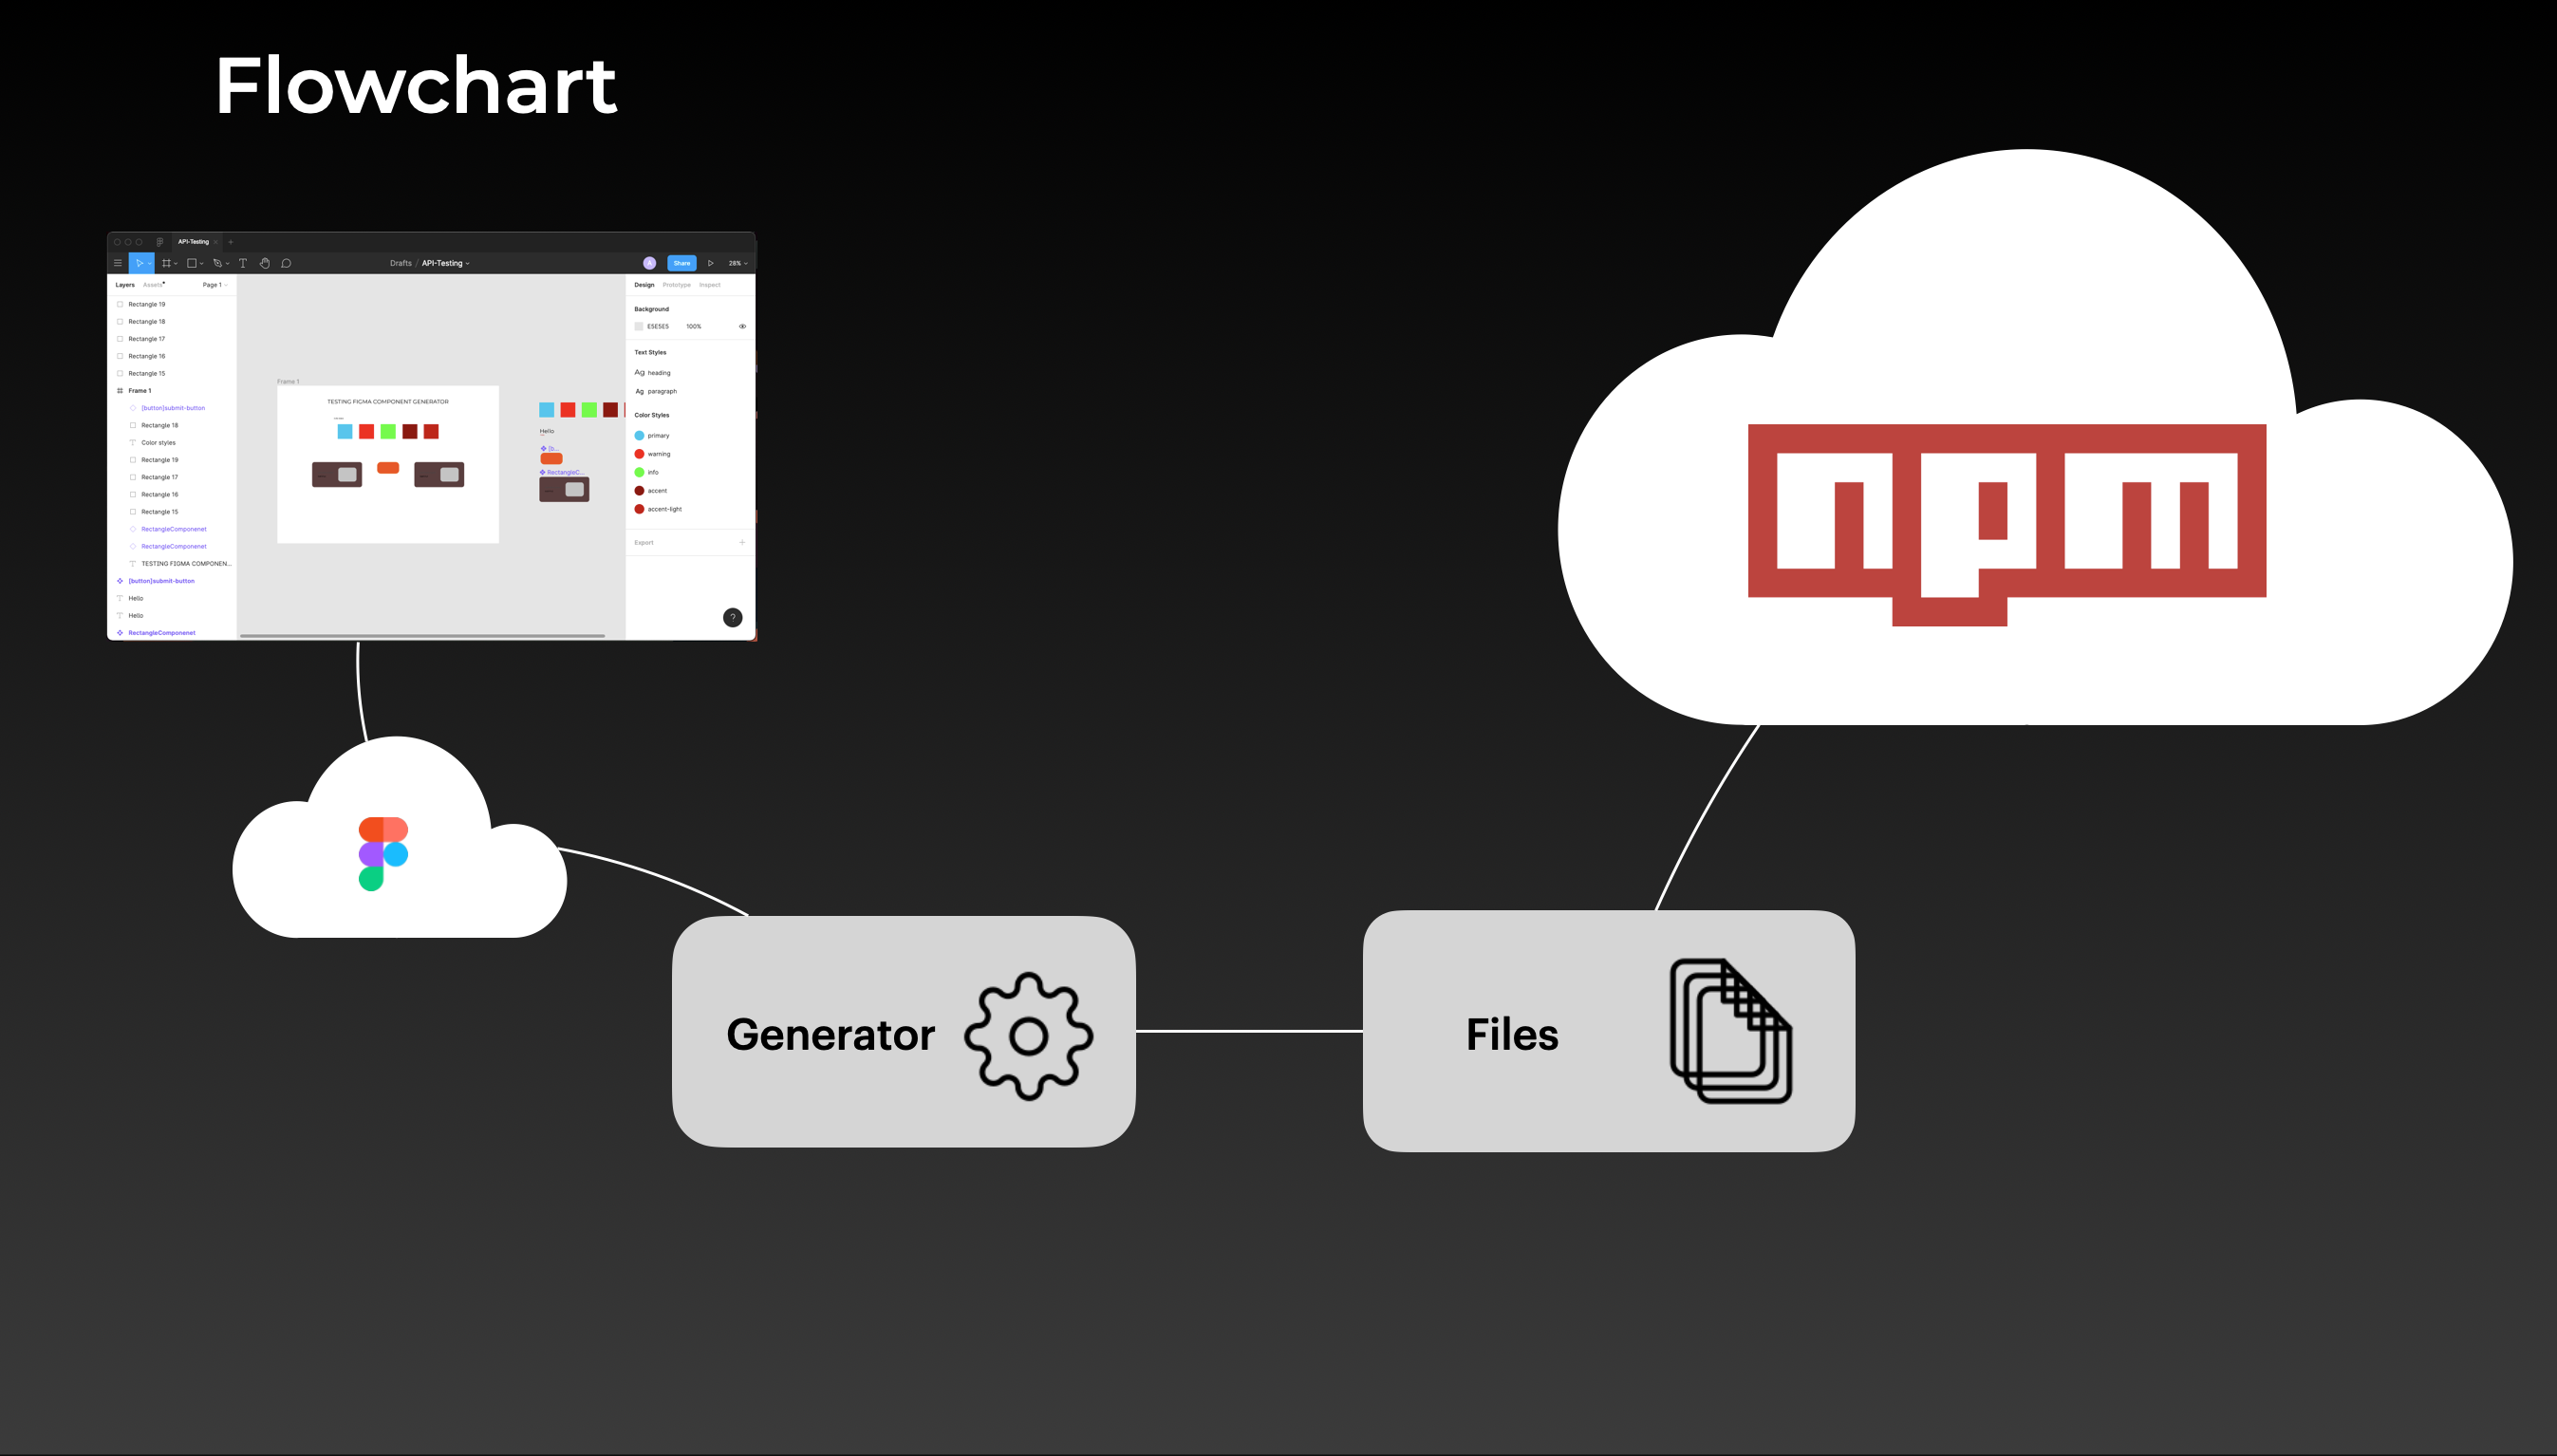
\includegraphics[width=0.8\linewidth]{images/flow.png}
  \caption{Chart over how data flows in the program}%
  \label{fig:flow}
\end{figure}



\subsection{Competitors}%
\label{sub:Competitors}
The idea of making a design program generate functional code is not new. For inspiration and to get a general knowledge of how these programs work we will look at two competitors in this field. 

\subsubsection{Webflow}
Webflow was founded in 2013 and is a product of the famous Y Combinator program. Webflow allows the user to design, create and publish a website all from their web application. Webflow is a visual editing tool. The user doesn't need to have any knowledge about programming since Webflow generates HTML, CSS, and JavaScript from the design. Most UI applications let the user move elements freely around the canvas. Webflow is a more static build tool where the elements in the design \textit{snap} in place. Most of the design is made through the control panel, which can be seen in figure \ref{fig:webflow}, and not on the canvas itself \cite{ResponsiveWebDesign}.

\begin{figure}[H]
  \centering
  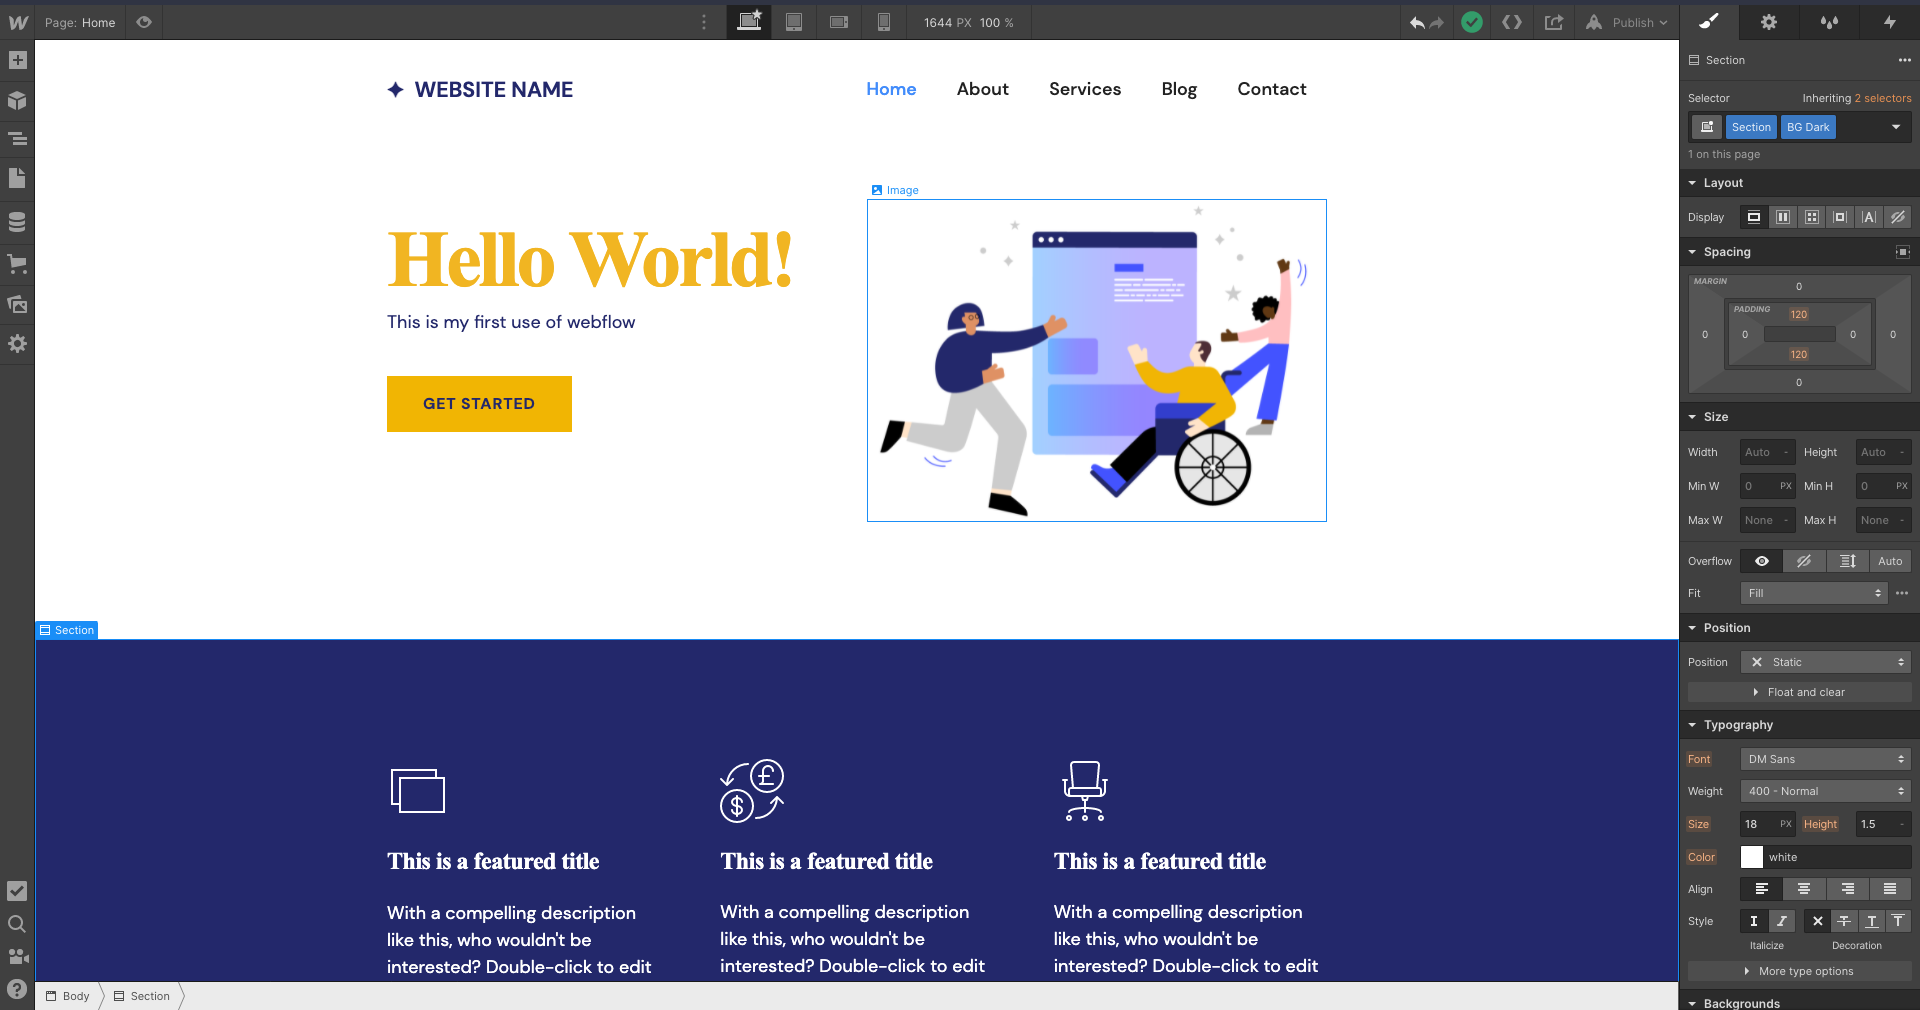
\includegraphics[width=0.8\linewidth]{images/webflow.png}
  \caption{Screenshot of Webflows UI \todo{Lägg till rätt referens för screenshots}}%
  \label{fig:webflow}
\end{figure}

\subsubsection{Visly}%
\label{ssub:Visly}
Visly was founded in 2018 and is very similar to Figma in how the user designs the product. Visly uses the design to create React components \cite{facebookincReactJavaScriptLibrary}. React is a component-based JavaScript framework made by Facebook. Visly essentially makes it possible to create these components visually. 

\begin{figure}[H]
  \centering
  \includegraphics[width=0.8\linewidth]{images/visly.png}
  \caption{ Screenshot of Vislys UI \todo{Lägg till rätt referens för screenshots}}%
  \label{fig:visly}
\end{figure}



% \subsubsection{Bravo}%
% \label{ssub:Bravo}

% Build Native IOS och Android apps with Figma. Think this can be the closest to the what I'm trying to do. 

\subsubsection{Competitors summery}%
\label{ssub:Comparison}

The disadvantages with both of these competitors are that they are locked with either a framework or a program. This is something that we want to avoid as far as possible because of the reason, stated in section \ref{ssub:Knowit Initial Requirements}, that Knowit wants to be able to use the program in all projects. Knowit uses the UI program Figma when designing UI's for their projects. Knowit is happy with the functionality within Figma and doesn't want to change program. Therefore the prototype must be built around Figma as a UI design platform.




